\chapter{Mathieu Moonshine}\label{ch:moonshine}

In \cref{ch:ellgenus} we expanded the elliptic genus of a K3 surface in characters of the
$N=4$ superconformal algebra and found that the multiplicities of the massive
representations are the integers $2A_n$ with $A_n=45,\,231,\,770,\,2277,\,5796,\dots$.
In \cref{ch:m24} we met the sporadic group $\Mtf$ of order $244\,823\,040$ and its
$26$ irreducible representations. This chapter is about the fact that these two lists are the
same list.\index{Mathieu moonshine}\index{moonshine!Mathieu} The question it answers is: what exactly has been observed, how much of it is a
coincidence that could be produced by small numbers, and which independent tests turn a
numerological remark into a structural statement? Along the way the student learns the one
technique that makes moonshine testable at all---replacing dimensions by characters and
asking whether the resulting functions have the modular behaviour that a conformal field
theory would force on them---and sees, at the end, exactly which pieces of the story are
arithmetic that a proof assistant can check, and which pieces remain a conjecture of this
programme or an open problem of the field.

Conventions. Throughout $q=\ee^{2\pi\ii\tau}$ and $y=\ee^{2\pi\ii z}$ with $\tau$ in the
upper half plane. The elliptic genus of a K3 sigma model is the Ramond--Ramond trace
\begin{equation}\label{eq:moonshine:ellgenus}
  Z(\tau,z)=\Tr_{RR}\,(-1)^{F_L+F_R}\,q^{L_0-\frac{c}{24}}\,\bar q^{\bar L_0-\frac{\bar c}{24}}\,
  y^{J_0},\qquad c=\bar c=6,
\end{equation}
where $J_0$ is the integer-valued $U(1)$ charge of the $N=2$ subalgebra, $J_0=2J^3_0$ in
terms of the $SU(2)$ Cartan generator used by Eguchi--Ooguri--Tachikawa
\source{EOT §1, ll.~44--56}. Our $Z$ is EOT's $Z_{\mathrm{ell}}$ and equals twice the
standard weak Jacobi form $\phi_{0,1}$; Gaberdiel--Hohenegger--Volpato work with
$\phi_{1A}:=\tfrac12 Z=\phi_{0,1}$ \source{GHV §2, ll.~153--170}. The symbol $A_n$ always
denotes the EOT coefficients $45,231,\dots$; GHV absorb a factor $2$ into their $A_n$
\source{GHV §3, ll.~540--545}, and \cref{sec:moonshine:conjugate} explains why the book does
not.

\section{The observation}\label{sec:moonshine:observation}

\subsection{The decomposition, recalled}

The K3 sigma model has $N=(4,4)$ superconformal symmetry with $c=6$, and its Ramond
sector Hilbert space decomposes into representations of the left-moving $N=4$ algebra
\cref{ch:ellgenus}. Two kinds of representation\index{N=4 superconformal algebra@$N=4$ superconformal algebra!characters} occur at $c=6$: the massless (BPS, short)
ones with $h=\tfrac14$ and isospin $\ell=0$ or $\ell=\tfrac12$, and the massive (non-BPS,
long) ones with $h>\tfrac14$ and $\ell=\tfrac12$. Their characters with $(-1)^F$ inserted
are \source{EOT §1, ll.~82--124}
\begin{align}
  \mathrm{ch}^{\hat R}_{h=\frac14,\ell=0}(\tau;z)&=\frac{\theta_1(\tau;z)^2}{\eta(\tau)^3}\,
    \mu(\tau;z),\qquad
  \mu(\tau;z)=\frac{-\ii\,\ee^{\pi\ii z}}{\theta_1(\tau;z)}\sum_{n\in\Z}
    \frac{(-1)^n q^{n(n+1)/2}\ee^{2\pi\ii nz}}{1-q^n\ee^{2\pi\ii z}},
    \label{eq:moonshine:masslesschar}\\
  \mathrm{ch}^{\hat R}_{h,\ell=\frac12}(\tau;z)&=q^{h-\frac38}\,
    \frac{\theta_1(\tau;z)^2}{\eta(\tau)^3}\qquad(h>\tfrac14).
    \label{eq:moonshine:massivechar}
\end{align}
The function $\mu$ is an Appell--Lerch sum\index{Appell--Lerch sum}\index{mock modular form}, not a modular form: this is the technical
reason why moonshine for K3 is harder than for the Monster, and we return to it in
\cref{sec:moonshine:twining}. The massless $\ell=0$ character has Witten index $1$,
$\mathrm{ch}^{\hat R}_{\frac14,0}(\tau;0)=1$ \source{EOT §1, ll.~98--104}. At the unitarity
bound $h=\tfrac14$ the massive character \eqref{eq:moonshine:massivechar} is not irreducible
but splits, $q^{-1/8}\theta_1^2/\eta^3=2\,\mathrm{ch}^{\hat R}_{\frac14,0}+
\mathrm{ch}^{\hat R}_{\frac14,\frac12}$ \source{EOT §1, ll.~140--150}.

The decomposition of the elliptic genus reads, in the two equivalent forms of EOT,
\begin{align}
  Z(\tau,z)&=24\,\mathrm{ch}^{\hat R}_{\frac14,0}(\tau;z)+\Sigma(\tau)\,
    \frac{\theta_1(\tau;z)^2}{\eta(\tau)^3},\qquad
    \Sigma(\tau)=-2q^{-1/8}\Bigl(1-\sum_{n\ge1}A_nq^n\Bigr),
    \label{eq:moonshine:decompSigma}\\
  Z(\tau,z)&=20\,\mathrm{ch}^{\hat R}_{\frac14,0}-2\,\mathrm{ch}^{\hat R}_{\frac14,\frac12}
    +2\sum_{n\ge1}A_n\,q^{n-\frac18}\frac{\theta_1(\tau;z)^2}{\eta(\tau)^3}
    \label{eq:moonshine:decomp}
\end{align}
\source{EOT §1, ll.~126--165}. The second form is obtained from the first by the splitting
identity; it exhibits the multiplicity of the massive representation of weight
$h=n+\tfrac14$ as $2A_n$, and the two massless multiplicities as $20$ and $-2$. Expanding
$\Sigma$, EOT tabulate \source{EOT eq.~(1.12), ll.~200--210}
\begin{equation}\label{eq:moonshine:An}
\begin{array}{c|ccccccccc}
 n & 1&2&3&4&5&6&7&8&9\\ \hline
 A_n & 45&231&770&2277&5796&13915&30843&65550&132825
\end{array}
\end{equation}
The $A_n$ are positive integers; their growth is governed by a Rademacher-type formula
$A_n\approx\frac{2}{\sqrt{8n-1}}\,\ee^{2\pi\sqrt{(n-1/8)/2}}$ which is accurate already for
small $n$ \source{EOT §1, ll.~212--226}.

\subsection{Twenty-six numbers}

The group $\Mtf$\index{Mathieu group M24@Mathieu group $M_{24}$!irreducible representations} has order $2^{10}\cdot3^3\cdot5\cdot7\cdot11\cdot23=244\,823\,040$,
$26$ conjugacy classes and hence $26$ irreducible representations, of dimensions
\source{EOT App.~A, ll.~330--349}
\begin{equation}\label{eq:moonshine:dims}
\begin{gathered}
 1,\;23,\;45,\;45,\;231,\;231,\;252,\;253,\;483,\;770,\;770,\;990,\;990,\;1035,\;1035,\;1035,\\
 1265,\;1771,\;2024,\;2277,\;3312,\;3520,\;5313,\;5796,\;5544,\;10395.
\end{gathered}
\end{equation}
Comparing \eqref{eq:moonshine:An} with \eqref{eq:moonshine:dims} one sees the observation
of Eguchi, Ooguri and Tachikawa \source{EOT §1, ll.~227--235}: \emph{$A_1,\dots,A_5$ are
each the dimension of an irreducible representation of $\Mtf$}, and the next two
coefficients are sums of such dimensions,
\begin{equation}\label{eq:moonshine:A6A7}
  A_6=13915=3520+10395,\qquad
  A_7=30843=10395+5796+5544+5313+2024+1771 .
\end{equation}
For $n\ge8$ decompositions still exist but are far from unique; and indeed
\eqref{eq:moonshine:A6A7} for $A_7$ is already not the decomposition EOT first proposed---it
was corrected in the second version of their paper after the twining-genus analysis of
\cref{sec:moonshine:twining} showed the original guess to be inconsistent
\source{EOT footnote~1, ll.~259--261}. This is the first lesson of the chapter: dimensions
alone cannot decide between competing decompositions; characters can.

\begin{historybox}[Monstrous moonshine]\index{moonshine!monstrous}\index{Monster group}
The observation was made in deliberate analogy with McKay and Thompson's remark that the
coefficients of the modular $J$-function, $J(q)=q^{-1}+196884q+21493760q^2+\dots$, are
sums of dimensions of irreducible representations of the Monster group. Conway and Norton
made it a conjecture about a graded Monster module $\bigoplus_iV_i$ with $\dim V_i$ the
coefficients of $J$; Frenkel, Lepowsky and Meurman then constructed that module as the
chiral algebra of a string on $\R^{24}/\Lambda_{\mathrm{Leech}}/\Z_2$
\source{EOT §1, ll.~237--256}. For K3 the graded vector space is given from the start---it
is the Hilbert space of the sigma model---and the missing piece is the group action
\source{EOT §1, ll.~264--268}.
\end{historybox}

\subsection{Conjugate pairs, real representations and the factor two}
\label{sec:moonshine:conjugate}

Of the $26$ irreducibles, exactly those of dimension $45$, $231$, $770$, $990$ and $1035$
come in complex-conjugate pairs\index{conjugate representations} $(\rho,\bar\rho)$; there is a third, real,
$1035$-dimensional representation, and every other irreducible is real
\source{EOT App.~A, ll.~352--356}. The multiplicity of the massive $N=4$ representation at
level $n$ is $2A_n$, not $A_n$, so the natural guess for the $\Mtf$-module $R_n$ at level $n$
is
\begin{equation}\label{eq:moonshine:Rn}
  R_1=\mathbf{45}\oplus\overline{\mathbf{45}},\quad
  R_2=\mathbf{231}\oplus\overline{\mathbf{231}},\quad
  R_3=\mathbf{770}\oplus\overline{\mathbf{770}},\quad
  R_4=\mathbf{2277}\oplus\mathbf{2277},\quad
  R_5=\mathbf{5796}\oplus\mathbf{5796},
\end{equation}
of dimensions $90,462,1540,4554,11592$ \source{GHV §3, ll.~527--560} (the extracted text
of GHV prints ``$1440$'' for $770+770$; it is $1540$). Real modules are
forced: the elliptic genus counts states of a Hilbert space with a real structure, so the
$\Mtf$-representation on each graded piece is self-conjugate, and a complex irreducible can
only occur together with its conjugate. This is also why the twining characters of conjugacy
classes that differ only on conjugate representations coincide
\source{GHV App.~A.2, ll.~1605--1610}.

\begin{pitfallbox}[$4554=2\cdot2277$, not $2277\oplus\overline{2277}$]
It is tempting to write every $R_n$ as $\rho\oplus\bar\rho$. For $n=4$ this is wrong:
$\mathbf{2277}$ is real, so $\overline{\mathbf{2277}}=\mathbf{2277}$ and $R_4$ is two
copies of one real irreducible. The distinction is invisible at the level of dimensions but
visible at the level of characters (the two summands contribute equal characters rather than
complex-conjugate ones). An earlier paper of this programme wrote
$4554=\mathbf{2277}\oplus\overline{\mathbf{2277}}$; the correction is recorded in
\texttt{docs/PAPER\_REVISION\_BRIEF\_2026\_09\_17.md}, item~3. The same document fixes the
convention $\mathcal A_n:=2A_n$ for the doubled multiplicities used in the older Lean
libraries, so that they do not clash with EOT's $A_n$.
\end{pitfallbox}

\subsection{Worked example: computing \texorpdfstring{$A_n$}{A\_n} from the Lerch sum}
\label{sec:moonshine:worked1}

The table \eqref{eq:moonshine:An} should not be taken on trust: pdf extraction garbles
numbers, and the whole chapter rests on them. Here is a route that reproduces all nine
values from \eqref{eq:moonshine:decompSigma} with exact rational arithmetic.

\emph{Step 1: specialize to $z=\tfrac12$.} Equation \eqref{eq:moonshine:decompSigma} holds
for every $z$, so
\begin{equation}\label{eq:moonshine:Sigmaformula}
  \Sigma(\tau)=Z(\tau,z)\,\frac{\eta(\tau)^3}{\theta_1(\tau;z)^2}-24\,\mu(\tau;z)
\end{equation}
is independent of $z$, and we may choose $z$ to make everything a $q$-series with rational
coefficients. At $z=\tfrac12$, i.e.\ $y=-1$, the product formulas
\source{GHV App.~A, ll.~1456--1478} give
$\theta_1(\tau;\tfrac12)=\theta_2(\tau)$, $\theta_2(\tau;\tfrac12)=0$,
$\theta_3(\tau;\tfrac12)=\theta_4(\tau)$, $\theta_4(\tau;\tfrac12)=\theta_3(\tau)$, where
$\theta_i(\tau):=\theta_i(\tau;0)$. In the Lerch sum \eqref{eq:moonshine:masslesschar} the
prefactor becomes $-\ii\ee^{\pi\ii/2}=1$ and $(-1)^n\ee^{2\pi\ii n/2}=1$, so
\begin{equation}\label{eq:moonshine:S}
  \mu(\tau;\tfrac12)=\frac{S(q)}{\theta_2(\tau)},\qquad
  S(q)=\sum_{n\in\Z}\frac{q^{n(n+1)/2}}{1+q^n}
  =\sum_{m\ge0}q^{m(m+1)/2}\Bigl[\frac1{1+q^m}+\frac{q^{m+1}}{1+q^{m+1}}\Bigr],
\end{equation}
where the second form pairs $n=m$ with $n=-1-m$. The first terms are
$S=\tfrac12+2q-2q^2+4q^3-\dots$.

\emph{Step 2: the elliptic genus at $z=\tfrac12$.} From
$Z=8\sum_{i=2,3,4}\theta_i(\tau;z)^2/\theta_i(\tau)^2$ \source{EOT eq.~(1.2), ll.~60--75}
and the specializations above,
\begin{equation}\label{eq:moonshine:Zhalf}
  Z(\tau,\tfrac12)=8\Bigl[\frac{\theta_4(\tau)^2}{\theta_3(\tau)^2}
  +\frac{\theta_3(\tau)^2}{\theta_4(\tau)^2}\Bigr]=16+512q+\dots,
\end{equation}
which has integer powers of $q$ only because the bracket is invariant under
$q^{1/2}\mapsto-q^{1/2}$, which exchanges $\theta_3$ and $\theta_4$. The constant $16$ is the
signature of K3 \source{EOT §1, ll.~78--80}; the $512$ is $20+128+216+128+20$, the
$q^1$ coefficient of $Z$ evaluated at $y=-1$ (odd powers of $y$ change sign), in agreement
with the expansion $Z=2y+20+2y^{-1}+q(20y^2-128y+216-128y^{-1}+20y^{-2})+O(q^2)$
\source{GHV eq.~(2.5), ll.~153--158}, which we also re-derived symbolically from the theta
products.

\emph{Step 3: strip the fractional powers.} Write $\theta_2(\tau)=2q^{1/8}P_2(q)$ and
$\eta(\tau)^3=q^{1/8}P_\eta(q)$ with
\[
  P_2=\prod_{n\ge1}(1-q^n)(1+q^n)^2=1+q+q^3+q^6+\dots,\qquad
  P_\eta=\prod_{n\ge1}(1-q^n)^3=1-3q+5q^3-7q^6+\dots
\]
(the first is $\tfrac12q^{-1/8}\sum_{n\in\Z}q^{(n+1/2)^2/2}$, the second is Jacobi's
$\sum_{n\ge0}(-1)^n(2n+1)q^{n(n+1)/2}$). Multiplying \eqref{eq:moonshine:Sigmaformula} by
$q^{1/8}$ gives
\begin{equation}\label{eq:moonshine:Sigmaq}
  q^{1/8}\,\Sigma(\tau)=Z(\tau,\tfrac12)\,\frac{P_\eta}{4P_2^2}-12\,\frac{S}{P_2},
\end{equation}
and \eqref{eq:moonshine:decompSigma} predicts that the right-hand side equals
$-2+2\sum_{n\ge1}A_nq^n$: every fractional power has cancelled, as it must.

\emph{Step 4: the first two coefficients by hand.} The series needed are
\[
  \frac{P_\eta}{4P_2^2}=\tfrac14-\tfrac54q+\tfrac94q^2-\dots,\qquad
  \frac{S}{P_2}=\tfrac12+\tfrac32q-\tfrac72q^2+\dots,\qquad
  Z(\tau,\tfrac12)=16+512q+4096q^2+\dots
\]
(for instance $P_2^{-2}=1-2q+3q^2-\dots$ and $(1-3q)(1-2q+3q^2)=1-5q+9q^2+\dots$;
$(\tfrac12+2q-2q^2)(1-q+q^2)=\tfrac12+\tfrac32q-\tfrac72q^2$). Collecting powers of $q$
on the right of \eqref{eq:moonshine:Sigmaq}:
\begin{align*}
 q^0:&\quad 16\cdot\tfrac14-12\cdot\tfrac12=4-6=-2,\\
 q^1:&\quad 16\cdot(-\tfrac54)+512\cdot\tfrac14-12\cdot\tfrac32=-20+128-18=90=2A_1,\\
 q^2:&\quad 16\cdot\tfrac94+512\cdot(-\tfrac54)+4096\cdot\tfrac14-12\cdot(-\tfrac72)
   =36-640+1024+42=462=2A_2 .
\end{align*}
The constant term is the statement that the massless multiplicities are $24-2\cdot2=20$
and $-2$; the next two reproduce $A_1=45$ and $A_2=231$ from nothing but theta functions
and the Lerch sum. A computer-algebra expansion of the exact right-hand side to order
$q^9$ (a symbolic check, not Tier A) gives
\[
  -2+90q+462q^2+1540q^3+4554q^4+11592q^5+27830q^6+61686q^7+131100q^8+265650q^9,
\]
which is $-2+2\sum_{n\le9}A_nq^n$ with precisely the nine values of
\eqref{eq:moonshine:An}. The lesson is methodological: derive the structure
\eqref{eq:moonshine:Sigmaq} by hand, check two coefficients by hand, and let the machine
do the rest---then cite the table with confidence.

\begin{physicsbox}[What the $A_n$ count]
The $2A_n$ massive $N=4$ multiplets at $h=n+\tfrac14$ are the left-moving BPS content of
type II string theory on K3: states that are $\tfrac12$-BPS with respect to the $N=2$
subalgebra, hence protected, hence countable by an index \source{GHV §3, ll.~500--505}.
Their exponential growth \eqref{eq:moonshine:An} is the growth of black-hole microstates:
for the $k$-th symmetric product of K3 the analogous coefficients grow exponentially with
a rate that at large $k$ becomes the D1--D5 black-hole entropy $S\approx2\pi\sqrt{kn}$
with $k=Q_1Q_5$\index{black hole!microstates and the elliptic genus}; the K3 elliptic genus
itself is the $Q_1=Q_5=1$ member of that family, a ``small'' black hole
\source{EOT §1, ll.~280--299}. Moonshine
says that these microstates fall into representations of $\Mtf$---a symmetry no one had
put in.
\end{physicsbox}

\section{Characters, not dimensions: twining genera}\label{sec:moonshine:twining}

\subsection{The idea}

If a finite group $G$ really acts on the Hilbert space of a conformal field theory,
commuting with the superconformal algebra, then for every $g\in G$ one may insert $g$ into
the trace \eqref{eq:moonshine:ellgenus}:
\begin{equation}\label{eq:moonshine:twining}
  Z_g(\tau,z)=\Tr_{RR}\,g\,(-1)^{F_L+F_R}\,q^{L_0-\frac c{24}}\,\bar q^{\bar L_0-\frac{\bar c}{24}}\,
  y^{J_0}
\end{equation}
\source{GHV eq.~(3.5), ll.~563--580}. This is the \emph{twining genus}\index{twining genus}
of $g$; it depends only on the conjugacy class of $g$.\index{McKay--Thompson series} Decomposing the Hilbert space into
$N=4$ representations as before, each multiplicity space is now a $G$-module, and the
twining genus is obtained from \eqref{eq:moonshine:decomp} by replacing each dimension by
the character of $g$ on that module:
\begin{equation}\label{eq:moonshine:twiningdecomp}
  Z_g(\tau,z)=\Tr_{\mathbf{23}\oplus\mathbf 1}(g)\,\mathrm{ch}^{\hat R}_{\frac14,0}
  -2\,\mathrm{ch}^{\hat R}_{\frac14,\frac12}
  +\sum_{n\ge1}\Tr_{R_n}(g)\,q^{n-\frac18}\frac{\theta_1(\tau;z)^2}{\eta(\tau)^3},
\end{equation}
where the $24$ massless states are assigned the permutation representation
$\mathbf{23}\oplus\mathbf 1$, the $-2$ is $-(\mathbf 1\oplus\mathbf 1)$, and $R_n$ are the
modules \eqref{eq:moonshine:Rn} \source{GHV §3, ll.~527--560}. For the identity element
this is \eqref{eq:moonshine:decomp}. The point of the construction is that the left-hand
side is a trace in a conformal field theory and therefore must transform well under a
congruence subgroup of $\SLZ$, while the right-hand side is computable, term by term, from
the character table---so a proposed decomposition can be \emph{falsified}. In monstrous
moonshine the same construction produces the McKay--Thompson series
\source{GHV §1, ll.~63--75}.

\subsection{Which modular group}

The standard orbifold argument\index{orbifold!boundary conditions}\index{congruence subgroup $\Gamma_0(N)$} \source{GHV §3.1, ll.~596--720} runs as follows. Label the
two cycles of the torus by elements of $\{\pm1\}\times\Mtf$: the NS twining character
$\chi_g$ carries $(-1,1)$ on one cycle and $(-1,g)$ on the other, the entries $-1$ recording
the NS sector and the absence of $(-1)^F$, the second entry the group element inserted in
the trace. A modular transformation
$\bigl(\begin{smallmatrix}a&b\\c&d\end{smallmatrix}\bigr)$ maps the pair of labels
$(h,g)$ to $(h^dg^c,\,g^ah^b)$; the twining character is mapped to itself (up to a phase)
whenever
\begin{equation}\label{eq:moonshine:Gammag}
  a+b\equiv c+d\equiv1\pmod 2,\qquad c\equiv0\pmod{o(g)},
\end{equation}
with $o(g)$ the order of $g$. The subgroup so defined contains
$\Gamma_g=\Gamma_\theta\cap\Gamma_0(o(g))$, where $\Gamma_\theta=\langle T^2,S\rangle$ and
$\Gamma_0(N)$ is the usual congruence subgroup with $c\equiv0\bmod N$. (One uses that
$\gcd(a,o(g))=1$ follows from \eqref{eq:moonshine:Gammag} and $ad-bc=1$, and that in
$\Mtf$ the element $g^a$ is then conjugate to $g$.) A function invariant under $\Gamma_g$ up
to a multiplier system is determined by finitely many of its $q$-coefficients, and the
smaller $o(g)$ the larger $\Gamma_g$ and the fewer coefficients one needs. This is the test:
compute the first few coefficients of $Z_g$ from \eqref{eq:moonshine:twiningdecomp} and the
character table, and ask whether they can be completed to a $\Gamma_g$-invariant function
\source{GHV §3.1, ll.~700--720}.

\subsection{NS characters and the reconstruction formulas}

GHV find it convenient to pass to the NS sector by half a unit of spectral flow\index{spectral flow},
$L_0\mapsto L_0+\ell J_0+\ell^2c/6$, $J_0\mapsto J_0+\ell c/3$ with $\ell=\tfrac12$, together
with a shift $z\mapsto z+\tfrac12$ that removes the $(-1)^F$ \source{GHV §2, ll.~172--190}:
\begin{equation}\label{eq:moonshine:flow}
  \chi(\tau,z)=\exp\Bigl[2\pi\ii\Bigl(\frac\tau4+z+\frac12\Bigr)\Bigr]\,
  \phi\Bigl(\tau,\,z+\frac\tau2+\frac12\Bigr),\qquad \phi=\tfrac12Z,
\end{equation}
and then set $z=0$. The resulting $\chi(\tau)$ is a modular function for $\Gamma_\theta$
with multiplier $-1$ on both generators (the index is $m=1$, odd)
\source{GHV eq.~(2.10), ll.~213--222}. For K3,
\begin{equation}\label{eq:moonshine:kappa}
  \chi_{1A}(\tau)=\kappa(\tau)=\Bigl(\frac{2\theta_4(\tau)}{\theta_2(\tau)}\Bigr)^2
  -\Bigl(\frac{2\theta_2(\tau)}{\theta_4(\tau)}\Bigr)^2
  =q^{-1/4}\bigl(1-20q^{1/2}-62q-216q^{3/2}-641q^2-\dots\bigr)
\end{equation}
\source{GHV eq.~(2.11), ll.~228--236}. We verified \eqref{eq:moonshine:flow} and
\eqref{eq:moonshine:kappa} numerically at a generic point $(\tau,z)$ with high-precision
theta functions, and the expansion symbolically; the leading term
$q^{-1/4}(1-20q^{1/2})$ is quick by hand from $\theta_2=2q^{1/8}(1+q+\dots)$ and
$\theta_4=1-2q^{1/2}+2q^2-\dots$: the first square gives $q^{-1/4}(1-4q^{1/2})$ and the
second $-16q^{1/4}=-16q^{-1/4}q^{1/2}$; Exercise~\ref{exo:moonshine:ns} continues the
expansion.

Nothing is lost by setting $z=0$. Because the four functions $\theta_i(\tau,z)^2$ span a
two-dimensional space, any index-one Jacobi form is fixed by its values at $z=0$ and
$z=\tfrac12$, and one has \source{GHV eqs.~(2.12)--(2.13) and (3.6)--(3.7), ll.~254--292
and 596--630}
\begin{align}
  \chi_g(\tau,z)&=\phi_g(\tau,0)\,\frac{\theta_4(\tau,z)^2}{\theta_2(\tau)^2}
    -\phi_g(\tau,\tfrac12)\,\frac{\theta_3(\tau,z)^2}{\theta_2(\tau)^2},
    \label{eq:moonshine:rec36}\\
  \phi_g(\tau,z)&=\phi_g(\tau,0)\,\frac{\theta_2(\tau,z)^2}{\theta_2(\tau)^2}
    +\phi_g(\tau,\tfrac12)\,\frac{\theta_1(\tau,z)^2}{\theta_2(\tau)^2},
    \label{eq:moonshine:rec37}
\end{align}
with $\phi_g=\tfrac12Z_g$ and the constant term
$\phi_g(\tau,0)=\tfrac12\Tr_{\mathbf{23}\oplus\mathbf1}(g)$, half the number of points
of $\{1,\dots,24\}$ fixed by $g$ \source{GHV eq.~(3.8), ll.~628--632}. Both formulas are
checked at $z=0$ and $z=\tfrac12$ by inspection: $\theta_2(\tau,\tfrac12)=0$,
$\theta_1(\tau,\tfrac12)=\theta_2(\tau)$, $\theta_3(\tau,\tfrac12)=\theta_4(\tau)$,
$\theta_4(\tau,\tfrac12)=\theta_3(\tau)$. (The pdf extraction of the source interchanges
the positions of $\theta_3$ and $\theta_4$ in \eqref{eq:moonshine:rec36}; the assignment
above is the one that reproduces \eqref{eq:moonshine:kappa} from
$\phi_{1A}(\tau,0)=12$ and $\phi_{1A}(\tau,\tfrac12)=4(\theta_4^2/\theta_3^2+
\theta_3^2/\theta_4^2)$, and the one we confirmed numerically.) Given
$\chi_g(\tau)=\chi_g(\tau,0)$ and the fixed-point count, \eqref{eq:moonshine:rec36} at
$z=0$ yields $\phi_g(\tau,\tfrac12)$, and \eqref{eq:moonshine:rec37} then yields the whole
twining genus.

\subsection{Closed forms for elements of small order}

For the classes of order at most six GHV found closed formulas that match the low-lying
coefficients and have the required modular behaviour \source{GHV eq.~(3.14), ll.~730--775}:
\begin{equation}\label{eq:moonshine:closed}
\begin{aligned}
  \chi_{2A}(\tau)&=4\,\frac{\theta_4(\tau)^2}{\theta_2(\tau)^2},&
  \chi_{2B}(\tau)&=4\,\frac{\theta_3(\tau)^2}{\theta_2(\tau)^2},&
  \chi_{3A}(\tau)&=\Bigl(\frac{\eta(\tau)}{\eta(3\tau)}\Bigr)^3
     \frac{\theta_3(3\tau)}{\theta_3(\tau)},\\
  \chi_{4A}(\tau)&=\Bigl(\frac{\eta(\tau)\,\eta(2\tau)}{\eta(\tau/2)\,\eta(4\tau)}\Bigr)^4,&
  \chi_{4B}(\tau)&=2\,\frac{\theta_3(2\tau)}{\theta_2(2\tau)},&
  \chi_{6A}(\tau)&=\Bigl(\frac{\eta(\tfrac32\tau)\,\eta(2\tau)}{\eta(\tfrac12\tau)\,\eta(6\tau)}\Bigr)^2,
\end{aligned}
\end{equation}
each normalized to begin with $1\cdot q^{-1/4}$; there are also expressions for $4C$ and
$5A$. Most of them coincide, after $\tau\mapsto\tau/4$, with McKay--Thompson series of the
Monster (for instance $\kappa(\tau)=T_{[8a]}(\tau/4)$ with
$T_{[8a]}=q^{-1}-20q-62q^3-216q^5-641q^7-\dots$, which the reader can match against
\eqref{eq:moonshine:kappa}), and for $2A$, $2B$ the match holds only up to signs
\source{GHV App.~A.1, ll.~1560--1600}. All are invariant under $\Gamma_g$ up to a multiplier
system, which is non-trivial in every case since $T^2$ acts by $-1$
\source{GHV §3.1, ll.~776--800}. The classes $3B$ and $6B$ resisted a closed form; their
first coefficients are tabulated \source{GHV App.~A.2, ll.~1605--1630}, and the replication
identities of \cref{sec:moonshine:replication} indicate that $3B$ too behaves well.

\subsection{Worked example: the \texorpdfstring{$2A$}{2A} twining genus against the
character table}\label{sec:moonshine:worked2}

Let us run the test ourselves for the class $2A$, in the direction opposite to GHV's: take
the closed form $\chi_{2A}$ from \eqref{eq:moonshine:closed}, reconstruct the twining
genus, expand, and compare with the characters of $2A$ on the modules
\eqref{eq:moonshine:Rn}. Two columns of the $\Mtf$ character table are needed; we transcribe
them from the table reproduced in GHV \source{GHV App., ll.~1928--2100} in the order of
\eqref{eq:moonshine:dims}:
{\small\begin{equation}\label{eq:moonshine:chars}
\begin{array}{r|rrrrrrrrrrrrr}
 \dim & 1&23&45&45&231&231&252&253&483&770&770&990&990\\
 \chi(2A)&1&7&-3&-3&7&7&28&13&35&-14&-14&-18&-18\\
 \chi(3A)&1&5&0&0&-3&-3&9&10&6&5&5&0&0\\[2pt]
 \dim &1035&1035&1035&1265&1771&2024&2277&3312&3520&5313&5796&5544&\!10395\\
 \chi(2A)&-21&-21&27&49&-21&8&21&48&64&49&-28&-56&-21\\
 \chi(3A)&0&0&0&5&16&-1&0&0&10&-15&-9&9&0
\end{array}
\end{equation}}
Transcription errors are the enemy here, so we checked both columns against the
orthogonality relations of character theory (standard; not checked against a source in this
book's library): $\sum_i\dim\rho_i\,\chi_i(g)=0$ holds for both columns, and
$\sum_i\chi_i(g)^2=|C_{\Mtf}(g)|$ gives $21504$ for $2A$ and $1080$ for $3A$, both of which
divide $|\Mtf|$, with quotients $11385$ and $226688$---the class sizes. A wrong entry would
almost certainly break one of the four identities.

\emph{Reconstruction.} The class $2A$ fixes $1+7=8$ of the $24$ points, so
$\phi_{2A}(\tau,0)=4$. Inserting $\chi_{2A}=4\theta_4^2/\theta_2^2$ into
\eqref{eq:moonshine:rec36} at $z=0$,
\[
  4\,\frac{\theta_4^2}{\theta_2^2}=4\,\frac{\theta_4^2}{\theta_2^2}
  -\phi_{2A}(\tau,\tfrac12)\,\frac{\theta_3^2}{\theta_2^2}
  \quad\Longrightarrow\quad \phi_{2A}(\tau,\tfrac12)=0,
\]
and \eqref{eq:moonshine:rec37} collapses to the remarkably simple
\begin{equation}\label{eq:moonshine:phi2A}
  \phi_{2A}(\tau,z)=4\,\frac{\theta_2(\tau,z)^2}{\theta_2(\tau)^2}
  =(y+2+y^{-1})+q\,(\dots)+\dots .
\end{equation}
Its constant term $y+2+y^{-1}$ sums to $4=\tfrac12\Tr_{\mathbf{23}\oplus\mathbf1}(2A)$,
distributed as $1+2+1$ over $J_0=1,0,-1$; compare $y+10+y^{-1}$ for the identity (half of
$2y+20+2y^{-1}$), where $12=1+10+1$. The $2A$ trace over the twenty states of charge zero
is thus $2$, i.e.\ they split $11+9$ between the eigenvalues $\pm1$.

\emph{Expansion.} Now specialize \eqref{eq:moonshine:twiningdecomp} to $z=\tfrac12$ exactly
as in \cref{sec:moonshine:worked1}, with $\Tr_{\mathbf{24}}(g)$ in place of $24$ and
$c_n(g):=\Tr_{R_n}(g)$ in place of $2A_n$:
\begin{equation}\label{eq:moonshine:cn}
  \sum_{n\ge1}c_n(g)\,q^n=2+Z_g(\tau,\tfrac12)\,\frac{P_\eta}{4P_2^2}
  -\Tr_{\mathbf{24}}(g)\,\frac{S}{2P_2}.
\end{equation}
For $g=1$ this is \eqref{eq:moonshine:Sigmaq} rearranged. For $g\in2A$ we have
$Z_{2A}(\tau,\tfrac12)=2\phi_{2A}(\tau,\tfrac12)=0$ and $\Tr_{\mathbf{24}}=8$, so
\begin{equation}\label{eq:moonshine:cn2A}
\begin{aligned}
  \sum_{n\ge1}c_n(2A)\,q^n&=2-4\,\frac{S}{P_2}
  =2-4\bigl(\tfrac12+\tfrac32q-\tfrac72q^2+7q^3-\dots\bigr)\\
  &=-6q+14q^2-28q^3+42q^4-56q^5+86q^6-138q^7+\dots
\end{aligned}
\end{equation}
(the coefficients beyond $q^3$ from the symbolic expansion). The prediction from the
character table is
\begin{align*}
 c_1&=2\chi_{45}(2A)=-6,& c_2&=2\chi_{231}(2A)=14,\\
 c_3&=2\chi_{770}(2A)=-28,& c_4&=2\chi_{2277}(2A)=42,\\
 c_5&=2\chi_{5796}(2A)=-56,&
 c_6&=2\bigl(\chi_{3520}+\chi_{10395}\bigr)(2A)=2(64-21)=86,
\end{align*}
and for the corrected $A_7$ of \eqref{eq:moonshine:A6A7},
$c_7=2(-21-28-56+49+8-21)=-138$. All seven agree. Note what has been tested: not only
that $A_1,\dots,A_5$ are dimensions, but that the specific irreducibles chosen---including the
choice of the real $\mathbf{2277}$ twice rather than some other combination of the same
total dimension, and the six-term decomposition of $A_7$---have characters on $2A$ that
assemble into a function with the modular behaviour of a $\Z_2$-twined trace. Repeating the
computation for $3A$ with the closed form in \eqref{eq:moonshine:closed}, $\Tr_{\mathbf{24}}(3A)=6$
and $\phi_{3A}(\tau,\tfrac12)=(3\theta_4^2-\chi_{3A}\theta_2^2)/\theta_3^2$, the symbolic
expansion gives $c_n(3A)=0,-6,10,0,-18,20,0$ for $n=1,\dots,7$, against the table's
$2\cdot(0,-3,5,0,-9,10+0,\,0-9+9-15-1+16)=(0,-6,10,0,-18,20,0)$. Again every coefficient
matches. The alternating signs of \eqref{eq:moonshine:cn2A} have a meaning: $2A$ acts on
the level-$n$ multiplicity space with $\tfrac12(2A_n+c_n)$ eigenvalues $+1$ and
$\tfrac12(2A_n-c_n)$ eigenvalues $-1$, so at $n=1$ the $90$ states split $42+48$.

\subsection{Replication}\label{sec:moonshine:replication}
\index{replication identities}\index{Hecke operator}
The second test is borrowed from the replication identities of monstrous moonshine. If
$\Mtf$ acts on the K3 theory, it acts diagonally on the symmetric orbifolds
$\mathrm{Sym}^p(\mathrm{K3})$, and the Hecke-transformed twining genera must be
\begin{equation}\label{eq:moonshine:hecke}
  (H_p\phi)_g(\tau,z)=\phi_{g^p}(p\tau,pz)+\sum_{l=0}^{p-1}\phi_g\Bigl(\frac{\tau+l}{p},z\Bigr),
\end{equation}
the first term from the untwisted sector with the cyclic permutation inserted (only
$u\otimes\cdots\otimes u$ contributes, with $g$ acting as $g^p$), the others from the twisted
sectors \source{GHV §3.2, ll.~830--870}. Translated into NS characters, the $p=2$ case
expresses the twining character $\chi^{(2)}_g$ of the Hecke part of $\mathrm{Sym}^2$ as
\begin{equation}\label{eq:moonshine:rep2}
  \chi^{(2)}_g(\tau)=\chi_{g^2}(2\tau,\tfrac12)+\phi_g(\tfrac\tau2,\tfrac12)-\phi_g(\tau,0),
\end{equation}
where $\chi_{g^2}(\tau,z)$ is the NS-flowed twining genus \eqref{eq:moonshine:flow} of
$g^2$ (the constant term is displayed by GHV as $-4$, $0$, $-3$ for $2A$, $2B$, $3A$, which
is $-\tfrac12\Tr_{\mathbf{24}}(g)$), and GHV find that the result is a polynomial in the
original twining character, for instance
\begin{equation}\label{eq:moonshine:rep2A}
  \chi^{(2)}_{2A}(\tau)=\chi_{2A}(\tau)^2+4,\qquad
  \chi^{(2)}_{2B}(\tau)=\chi_{2B}(\tau)^2-12,\qquad
  \chi^{(2)}_{3A}(\tau)=\chi_{3A}(\tau)^2,
\end{equation}
with analogues for $3B$, $4A$--$4C$, $5A$, $6A$, $7A$ \source{GHV eqs.~(3.17)--(3.21),
ll.~870--975}. We verified \eqref{eq:moonshine:rep2}--\eqref{eq:moonshine:rep2A} for $2A$
and $3A$ numerically at a generic $\tau$, using the closed forms \eqref{eq:moonshine:closed}
and the reconstruction \eqref{eq:moonshine:rec36}--\eqref{eq:moonshine:rec37}; for $2A$ the
middle term of \eqref{eq:moonshine:rep2} vanishes identically, so the identity reads
$\chi_{1A}(2\tau,\tfrac12)-4=16\,\theta_4(\tau)^4/\theta_2(\tau)^4+4$. Unlike the Monster case the twining characters are not Hauptmoduls, so
inhomogeneous terms (proportional to other McKay--Thompson series) can appear on the right
\source{GHV §4, ll.~1425--1430}. The identities hold in every case examined and give
independent evidence that even the classes without closed forms, such as $3B$ and $7A$,
have good modular properties \source{GHV §3.2, ll.~895--905}.

\section{Geometry: Mukai's theorem and the puzzle}\label{sec:moonshine:geometry}

\subsection{Why \texorpdfstring{$\Mtf$}{M24} and K3 belong together at all}

The group $\Mtf$ can be defined in a way a string theorist finds natural
\source{EOT App.~B, ll.~951--982}. Take the root lattice $A_1^{24}$, whose generators have
square $2$, inside its dual $(A_1^*)^{24}$, whose generators have square $\tfrac12$. An even
unimodular lattice $N$ with $A_1^{24}\subset N\subset(A_1^*)^{24}$ is specified by the
subspace $\mathcal G=N/A_1^{24}\subset(\Z_2)^{24}$: unimodularity forces
$\dim\mathcal G=12$, evenness forces every element of $\mathcal G$ to have weight divisible
by $4$, and demanding that the only vectors of square $2$ in $N$ be the roots of $A_1^{24}$
forbids weight-$4$ words. These conditions determine $\mathcal G$ uniquely: it is the
extended binary Golay code\index{Golay code}\index{Niemeier lattice}, and $\Mtf$ is its automorphism group inside
$S_{24}$. The lattice $N$ is a Niemeier lattice, and the chiral $c=24$ theory built on it has
$\Mtf$ as a discrete symmetry. The link to K3 is that $H^*(\mathrm{K3},\Z)$ with the Mukai
pairing (\cref{ch:mukai}) is also even and unimodular of rank $24$, of signature $(4,20)$
\source{EOT App.~B, ll.~983--990}.

Now let $G$ be a finite group of automorphisms of a K3 surface $X$ preserving the holomorphic
two-form (\emph{symplectic} automorphisms\index{symplectic automorphism}\index{K3 surface!symplectic automorphisms}). Let $\Lambda^G$ be the $G$-invariant part of
the Mukai lattice and $\Lambda_G$ its orthogonal complement. Since $G$ fixes $H^0$, $H^4$,
$H^{2,0}$, $H^{0,2}$ and the K\"ahler class, $\Lambda^G$ has rank at least $5$, so
$\Lambda_G$ has rank at most $19$; and $\Lambda_G$ lies in the primitive part of $H^{1,1}$,
hence is negative definite and, by a result of Nikulin, embeds into the Niemeier lattice
$N$. This makes $G$ a subgroup of $\Mtf$ whose action on $24$ points has at least five
orbits; conversely, the global Torelli theorem produces a K3 surface with symmetry $G$ from
any subgroup of $\Mtf$ with at least five orbits \source{EOT App.~B, ll.~991--1003}. The
precise statement is Mukai's theorem, which Huybrechts states with $M_{23}$
\source{Huy ch.~15 Thm.~3.1, ll.~14549--14560}:

\begin{theorem}[Mukai]\label{thm:moonshine:mukai}\index{Mukai's theorem}\index{Mathieu group M23@Mathieu group $M_{23}$}\TL\;
For a finite group $G$ the following are equivalent: (i) $G$ is isomorphic to a subgroup of
$\mathrm{Aut}_s(X)$ for some complex projective K3 surface $X$; (ii) there is an injection
$G\hookrightarrow M_{23}$ such that the induced action on $\Omega=\{1,\dots,24\}$ has at least
five orbits. There are exactly $11$ maximal such groups, of orders
$48,72,120,168,192,288,360,384,960$ (some occurring twice), all realized on explicit
quartics, complete intersections and double covers.
\end{theorem}

Here $M_{23}=\mathrm{Stab}(e_{24})\subset\Mtf$ is the stabilizer of a point, of index $24$
and order $|M_{23}|=10\,200\,960=2^7\cdot3^2\cdot5\cdot7\cdot11\cdot23$
\source{Huy ch.~15, ll.~14641--14645}. Any subgroup with a fixed point on $\Omega$ is
conjugate into $M_{23}$, which is why EOT's ``subgroup of $\Mtf$ with $\ge5$ orbits'' and
Huybrechts' ``subgroup of $M_{23}$ with $\ge5$ orbits'' say the same thing. The Fermat
quartic $X^4+Y^4+Z^4+W^4=0$ is the example EOT give: its symplectic group
$(\Z_4)^2\rtimes S_4$ has order $384=2^7\cdot3$ and splits $\Omega$ into orbits of
lengths $1,1,2,4,16$ \source{EOT App.~B, ll.~1004--1007}; $384$ is indeed one of the eleven
maximal orders in \cref{thm:moonshine:mukai} (\cref{fig:moonshine:orbits}).

\begin{figure}[ht]
\centering
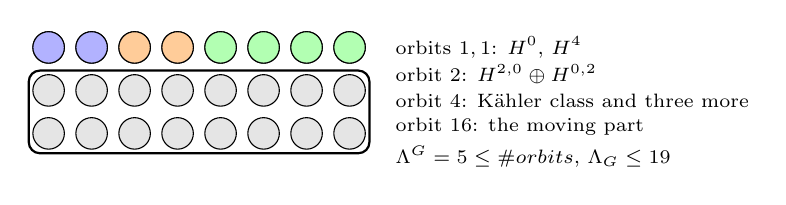
\begin{tikzpicture}[scale=0.42,every node/.style={font=\scriptsize}]
  \foreach \i in {0,...,23}{
    \pgfmathsetmacro{\x}{mod(\i,8)}
    \pgfmathsetmacro{\y}{-int(\i/8)}
    \node[circle,draw,fill=black!10,minimum size=4mm,inner sep=0pt] (p\i) at (1.3*\x,1.3*\y) {};
  }
  \node[circle,draw,fill=blue!30,minimum size=4mm,inner sep=0pt] at (p0) {};
  \node[circle,draw,fill=blue!30,minimum size=4mm,inner sep=0pt] at (p1) {};
  \node[circle,draw,fill=orange!40,minimum size=4mm,inner sep=0pt] at (p2) {};
  \node[circle,draw,fill=orange!40,minimum size=4mm,inner sep=0pt] at (p3) {};
  \foreach \i in {4,5,6,7}{\node[circle,draw,fill=green!30,minimum size=4mm,inner sep=0pt] at (p\i) {};}
  \draw[rounded corners,thick] (-0.6,-3.2) rectangle (9.7,-0.7);
  \node[anchor=west] at (10.2,0) {orbits $1,1$: $H^0$, $H^4$};
  \node[anchor=west] at (10.2,-0.8) {orbit $2$: $H^{2,0}\oplus H^{0,2}$};
  \node[anchor=west] at (10.2,-1.6) {orbit $4$: K\"ahler class and three more};
  \node[anchor=west] at (10.2,-2.4) {orbit $16$: the moving part};
  \node[anchor=west] at (10.2,-3.3) {$\rk\Lambda^G=5\le\#\text{orbits}$, $\rk\Lambda_G\le19$};
\end{tikzpicture}
\caption{The $24$ points of $\Omega$ under the symplectic group of order $384$ of the Fermat
quartic, in orbits of length $1,1,2,4,16$. Each orbit contributes one invariant vector, so
the number of orbits bounds $\rk\Lambda^G$ from below; a symplectic group must have at least
five orbits because $H^0,H^4,H^{2,0},H^{0,2}$ and the K\"ahler class are fixed. The
assignment of individual cohomology classes to orbits in the picture is schematic; only the
counts are meaningful.}
\label{fig:moonshine:orbits}
\end{figure}

\subsection{Fixed points, the Witten index, and which classes are geometric}

The constant term of the twining genus is a piece of classical geometry. At $z=0$ the
twining genus reduces to $\Tr_{\mathbf{24}}(g)=\Tr_{H^*(X)}(g^*)$ (all cohomology of K3
sits in even degree, so the sign $(-1)^{F_L+F_R}$ is $+1$ on every Ramond ground state), and
for a symplectic automorphism $f$ of finite order the topological Lefschetz formula turns
this into the number of fixed points, $\sum_i(-1)^i\Tr f^*|_{H^i(X,\Q)}=|\mathrm{Fix}(f)|$
\source{Huy ch.~15 eq.~(1.2), ll.~14105--14108}. Mukai's fixed-point count\index{Lefschetz fixed-point formula}\index{fixed points of a symplectic automorphism} states
\source{Huy ch.~15 Cor.~1.5, ll.~14032--14040}
\begin{equation}\label{eq:moonshine:fix}
  |\mathrm{Fix}(f)|=\frac{24}{n}\prod_{p\mid n}\Bigl(1+\frac1p\Bigr)^{-1},\qquad n=|f|,
\end{equation}
which depends only on the order, and lies between $1$ and $8$; the proof uses the
holomorphic Lefschetz formula, whose left side equals $2$ because $f$ acts trivially on
$H^0(X,\mathcal O)$ and $H^2(X,\mathcal O)$. A Nikulin involution\index{Nikulin involution} ($n=2$) has exactly
eight fixed points \source{Huy ch.~15 §4, ll.~14913--14915}.

Compare with the character table. The number of points of $\Omega$ fixed by $g$ is
$1+\chi_{\mathbf{23}}(g)$, which from the $23$-row of the table (the second row of
\eqref{eq:moonshine:chars}, continued across all classes) equals
$8,6,4,4,2,3,2$ for the classes $2A,3A,4B,5A,6A,7A,8A$ and $0$ for $2B,3B,4A,4C,12B,\dots$
\source{GHV App., ll.~1928--1970}. Evaluating \eqref{eq:moonshine:fix} at
$n=2,3,4,5,6,7,8$ gives $8,6,4,4,2,3,2$---exactly the fixed-point counts of the classes
that lie in $M_{23}$, which are those with a fixed point on $\Omega$
\source{GHV §3.1, ll.~805--812}. The other classes fix no point of $\Omega$ and thus cannot
be the action of a symplectic automorphism, whose fixed set is non-empty by
\eqref{eq:moonshine:fix}. So the twining genera fall into two families:
\begin{itemize}[leftmargin=*]
\item classes in $M_{23}$ ($1A,2A,3A,4B,5A,6A,7A,8A,\dots$): $Z_g(\tau,0)=|\mathrm{Fix}(g)|>0$;
  these can be realized geometrically, and for them the twining genus is the equivariant
  elliptic genus of a K3 surface with a symplectic automorphism;
\item classes not in $M_{23}$ ($2B,3B,4A,4C,\dots$): $\Tr_{\mathbf{23}\oplus\mathbf1}(g)=0$,
  so by \eqref{eq:moonshine:rec36}--\eqref{eq:moonshine:rec37}
  \[
    \phi_g(\tau,z)=\phi_g(\tau,\tfrac12)\,\frac{\theta_1(\tau,z)^2}{\theta_2(\tau)^2}
    =-\chi_g(\tau)\,\frac{\theta_1(\tau,z)^2}{\theta_3(\tau)^2}
  \]
  \source{GHV eq.~(3.15), ll.~812--822}; these have no fixed points and no realization as
  automorphisms of a K3 surface.
\end{itemize}
GHV note that apart from this simplification they see no difference in behaviour between
the two families \source{GHV §3.1, ll.~822--826}. That is the puzzle.

\subsection{The puzzle}\label{sec:moonshine:puzzle}

The observation and its tests say that the graded space of $N=2$ half-BPS states of the K3
sigma model looks, coefficient by coefficient, like an $\Mtf$-module. Geometry says that
no K3 surface has more than a group of order $960$ of symplectic automorphisms, and that
these groups never contain the classes outside $M_{23}$; EOT already remark that $G$
``cannot be $\Mtf$ itself'' since a geometric action fixes at least five classes
\source{EOT App.~B, ll.~996--999}. Their proposed way out is that automorphism groups at
isolated points of the moduli space might be ``enhanced to $\Mtf$ over the whole of moduli
space when we consider the elliptic genus'' \source{EOT §1, ll.~271--276}: the elliptic
genus is constant on the connected moduli space of K3 sigma models (\cref{ch:stringsk3}),
so a symmetry visible only at special points might still organize the index. The library of
this book does not contain the later literature on the symmetry groups of K3 sigma models,
so we state its outcome as standard, not checked against a source in this book's library:
the symmetry group of any individual K3 sigma model\index{K3 sigma model!symmetries} is a subgroup of the Conway group\index{Conway group}
$\mathrm{Co}_0$, and none of them contains $\Mtf$. Thus the $\Mtf$ action is not the symmetry
of any one point in moduli space, and where it comes from remains open.

\begin{pitfallbox}[Small numbers make coincidences]
The dimensions of $\Mtf$-irreducibles below $10^4$ are dense enough that many integers
of that size are sums of a few of them; GHV stress this ``certain amount of arbitrariness''
\source{GHV §1, ll.~63--68}. The observation for $A_1,\dots,A_5$ has content because each
is a \emph{single} irreducible dimension (not a sum), and because five hits in a row among
$26$ values is unlikely by chance; the decompositions of $A_6$, $A_7$ have content only
after the twining test. A claim of the form ``$N$ is a sum of $\Mtf$ dimensions'' for a
single large $N$ has essentially no content. The same caution applies to any numerology in
this book, including the ratio $77/60$ discussed in \cref{sec:moonshine:lean}.
\end{pitfallbox}

\section{What is known and what is open}\label{sec:moonshine:status}

At the time of the two source papers the situation was: the observation (EOT); closed
forms for the twining characters of about half the conjugacy classes, all of the form
required by the orbifold argument; the corrected decomposition of $A_7$; replication
identities for $p=2,3,5$ tested in many examples; and the expectation that
the space of half-BPS states carries an $\Mtf$ action which should extend to the BPS
algebra of Harvey and Moore, in analogy with the Monster Lie algebra
\source{GHV §4, ll.~1419--1445}. GHV list as the next step finding closed forms for all
twining characters, presumably by more refined techniques than ``guessing and confirming''.

What happened afterwards is standard, not checked against a source in this book's
library, and we record it only in outline so that the student knows where the story stands:
the remaining twining genera were determined (Cheng; Gaberdiel, Hohenegger and Volpato;
Eguchi and Hikami), and Gannon proved that the resulting virtual $\Mtf$-modules are honest
modules, i.e.\ that all the multiplicities decompose into non-negative integer combinations
of irreducibles. That settles the \emph{existence} of the graded $\Mtf$-module. Still open,
as far as the sources of this book go, are the two questions EOT posed on their first
page: the reason for the action, and a construction of it on the K3 Hilbert space
comparable to the Frenkel--Lepowsky--Meurman construction for the Monster.

\begin{remark}[What this programme adds, and what it does not]\label{rem:moonshine:programme}
The Lean libraries described in the next section formalize the \emph{arithmetic} of
\cref{sec:moonshine:observation}: that the listed $A_n$ are entries and sums of entries of the
listed table, and that the table satisfies Burnside's identity. They do not formalize theta
functions, Lerch sums, $N=4$ characters, the twining test, or Gannon's theorem; those
remain \TL. The ``BPS ratio'' $77/60$ that several of the older libraries carry is a
naming of this programme, \TC, and is discussed as such below.
\end{remark}

\section{What the machine has checked}\label{sec:moonshine:lean}

Five Lean files touch this chapter. One of them (\lean{DualScaleStream2/Moonshine/EOT.lean})
formalizes the arithmetic of the observation against a certified table; three carry the
``BPS ratio'' of this programme; the fifth is unrelated to moonshine and sits in the
\lean{Moonshine} namespace by accident of history. All theorems below depend only on
\lean{propext}, \lean{Classical.choice} and \lean{Quot.sound}.

\subsection{The table and the observation}

The dimensions \eqref{eq:moonshine:dims} live in Stream~1 as a literal function on
\lean{Fin 26}, in EOT's order, guarded by Burnside's identity:
\begin{leancode}
def M24RepDim : Fin 26 → ℕ
  | ⟨0, _⟩ => 1
  | ⟨1, _⟩ => 23
  | ⟨2, _⟩ => 45
  ...
  | ⟨25, _⟩ => 10395
  | ⟨n + 26, h⟩ => absurd h (by omega)

theorem M24_order : (244823040 : ℕ) = 2^10 * 3^3 * 5 * 7 * 11 * 23 := by ...

theorem M24RepDim_sum_sq : (∑ i : Fin 26, M24RepDim i ^ 2) = 244823040 := by ...
\end{leancode}
(\lean{StringTheoryFormalization/StringDynamics/MathieuM24.lean}.) The table had once been
mistyped---two entries duplicated, two missing---and the sum of squares then came out as
$351\,061\,029$; the theorem \lean{M24RepDim\_sum\_sq} now makes such a slip a compile
error. Burnside's $\sum_i(\dim\rho_i)^2=|G|$ itself is \TL; the equality of the two
numerals is \TA.

\begin{leanbox}[In Lean: the first five coefficients are irreducible dimensions]
\begin{leancode}
def eotA : Fin 9 → ℕ := ![45, 231, 770, 2277, 5796, 13915, 30843, 65550, 132825]

theorem first_five_are_irreps :
    ∀ n : Fin 5, ∃ i : Fin 26, M24RepDim i = eotA (Fin.castLE (by norm_num) n) := by ...

theorem A6_decomposition :
    eotA 5 = M24RepDim 21 + M24RepDim 25 := rfl

theorem A7_decomposition :
    eotA 6 = M24RepDim 25 + M24RepDim 23 + M24RepDim 24 + M24RepDim 22 +
      M24RepDim 18 + M24RepDim 17 := rfl

theorem A6_not_irrep : ∀ i : Fin 26, M24RepDim i ≠ eotA 5 := by ...
\end{leancode}
\textbf{Reading.} \lean{eotA} is the literal list \eqref{eq:moonshine:An}. For each of the
first five indices there exists an index into the $26$-entry table with the same value (an
existence statement with explicit witnesses $2,4,9,19,23$, i.e.\ $45,231,770,2277,5796$).
The sixth and seventh entries equal the specific sums \eqref{eq:moonshine:A6A7} of table
entries. No table entry equals $13915$, so the decomposition of $A_6$ is not vacuous.
\textbf{Proof idea.} \lean{fin\_cases} on the finite index and \lean{rfl} on literal
naturals; \lean{A6\_not\_irrep} is a $26$-way case split closed by \lean{decide}.
\textbf{What is not proved.} That $\Mtf$ acts on anything; that the $A_n$ are coefficients
of the elliptic genus (that is \eqref{eq:moonshine:Sigmaq}, a statement about theta
functions, \TL); anything about $A_8,A_9$ beyond their listing. \textbf{Tier} \TA\ for the
arithmetic, \TL\ for its meaning.
\end{leanbox}

\subsection{The ``BPS ratio'' \texorpdfstring{$77/60$}{77/60}}
\index{BPS ratio (this programme)}\index{arithmetic shadow}
Three older libraries define the doubled multiplicities and a ratio built from them:
\begin{leancode}
-- DualScaleM24Formalization/Moonshine/MathieuRigidity.lean
def dimA1 : Nat := 90
def dimA2 : Nat := 462
def dimA3 : Nat := 1540
theorem dimA1_decomposition : dimA1 = 45 + 45 := by decide
def numSupercharges : Nat := 4
def rBPSNum : Nat := 77
def rBPSDen : Nat := 60
theorem r_bps_cross_multiplication :
    dimA2 * rBPSDen = (numSupercharges * dimA1) * rBPSNum := by decide
theorem r_bps_is_irreducible : Nat.gcd rBPSNum rBPSDen = 1 := by decide
theorem sym2_A1_dimension_is_4095 : dimSym2A1 = 4095 := by decide

-- DualScaleValidation/UseCase2_MoonshineBPS.lean
theorem bps_cross_multiplication_lock :
    dim_A2 * 60 = 27720 ∧ (4 * dim_A1) * 77 = 27720 := by ...
theorem bps_lock_exact_equality : dim_A2 * 60 = (4 * dim_A1) * 77 := rfl
theorem bps_ratio_coprime : Nat.gcd 77 60 = 1 := by decide
theorem m24_order_divisible_by_bps_lock :
    order_M24 = bps_character_lock * 8832 := rfl

-- StringTheoryFormalization/StringDynamics/BPSMultiplicities.lean
def bpsRatio : ℚ := 77 / 60
theorem bps_ratio_reduced : bpsRatio.num = 77 ∧ bpsRatio.den = 60 := by ...
theorem bps_ratio_pos : (0 : ℚ) < bpsRatio := by ...
noncomputable def bpsMultiplicity (n : ℕ) : ℝ :=
  Real.exp (4 * Real.pi * Real.sqrt n) / (n : ℝ) ^ (3 / 2 : ℝ)
\end{leancode}

\begin{leanbox}[In Lean: what the ``lock'' theorems literally say]
\textbf{Reading.} $462\cdot60=27720=(4\cdot90)\cdot77$; $\gcd(77,60)=1$;
$244\,823\,040=27720\cdot8832$; $\binom{91}{2}=4095$; the rational literal $77/60$ has
numerator $77$, denominator $60$ and is positive. Every one of these is a true statement
about specific integers, closed by \lean{decide}, \lean{rfl} or \lean{norm\_num}.
\textbf{Where $77/60$ comes from.} $A_2/(4A_1)=231/180=77/60$, equivalently
$\mathcal A_2/(4\mathcal A_1)$ with the doubled multiplicities; the ``$4$'' is called the
number of supercharges in the docstrings. The identity is recorded in this programme's
\texttt{LL.md} (l.~405); no source in the book's library contains it.
\textbf{What is not proved.} Nothing connects \lean{bpsRatio} to \lean{M24RepDim} or to
\lean{eotA} inside Lean; \lean{dimA1}, \lean{dim\_A1}, \lean{rBPSNum} are bare literals.
The definition \lean{bpsMultiplicity} is a formula with no theorem about it---not
positivity, not a growth rate, not a relation to \eqref{eq:moonshine:An}---and its
docstring's attribution to a Hardy--Ramanujan asymptotic is not pinned to a source; the
actual asymptotic of the $A_n$ is EOT's Rademacher-type formula quoted after
\eqref{eq:moonshine:An}, with a different exponent. \textbf{Tier} \TA\ for the integer
identities; \TC\ for the words ``BPS ratio'', ``character lock'' and ``rigidity''.
\end{leanbox}

\begin{pitfallbox}[``Rigid under moduli deformation'' is empty for an integer]
The docstrings of these files say that because $27720$ is an integer the ratio $77/60$
``cannot continuously deform under any moduli variation of $\KT$''. Every integer is
invariant under continuous deformation; the statement has no content beyond the fact that
BPS multiplicities are integers, which is the standard reason the elliptic genus is a
deformation invariant (\cref{ch:ellgenus}). Likewise $|\Mtf|/27720=8832$ is a divisibility
fact about the numeral $2^{10}3^3\cdot5\cdot7\cdot11\cdot23$ and $27720=2^3\cdot3^2\cdot5\cdot7\cdot11$;
it says nothing about a decomposition of any Hilbert space into ``$8832$ copies'' of
anything. When a student meets a theorem whose proof is \lean{decide}, the right question is
always: what would have to be true for this to be \emph{false}? If the answer is ``a
different integer'', the theorem is a table lookup.
\end{pitfallbox}

\subsection{A file in the wrong drawer}

\lean{DualScaleM24Formalization/Moonshine/GysinBEMSequence.lean} is listed with this chapter
because its namespace is \lean{SocrateAI.Moonshine.GysinSequence}; its content is
topological T-duality for circle bundles (the Bouwknegt--Evslin--Mathai exchange
$c_1(\hat E)=\pi_*H$, $\hat\pi_*\hat H=c_1(E)$), which belongs with \cref{ch:buscher} and
\cref{ch:dbranes}, and it has nothing to do with $\Mtf$. For completeness:
\begin{leancode}
structure BEMDualPair (cr : CohomologyRing) where
  E : CircleBundle cr
  E_dual : CircleBundle cr
  H : Int
  H_dual : Int
  bem_dual_c1 : E_dual.c1 = E.pi_push H
  bem_dual_H  : E_dual.pi_push H_dual = E.c1

theorem bem_derived_exchange (cr : CohomologyRing) (pair : BEMDualPair cr) :
    pair.E_dual.c1 = pair.E.pi_push pair.H ∧
    pair.E_dual.pi_push pair.H_dual = pair.E.c1 := ⟨pair.bem_dual_c1, pair.bem_dual_H⟩

theorem bem_characteristic_vanishing (cr : CohomologyRing) (pair : BEMDualPair cr)
    (x : Int) :
    x * pair.E.c1 * pair.E_dual.c1 = x * pair.E.c1 * pair.E.pi_push pair.H := by ...
\end{leancode}
\textbf{Reading.} Cohomology groups are modelled by single integers and the Gysin maps by
arbitrary functions $\Z\to\Z$; the BEM relations are \emph{fields} of the structure, i.e.\
hypotheses. The first theorem returns those two hypotheses as a conjunction; the second
rewrites $c_1(\hat E)$ by the first hypothesis inside a product. Neither the vanishing
$c_1(E)\smile c_1(\hat E)=0$ nor exactness of the Gysin sequence is proved (the exactness
field \lean{h\_exact\_push\_pull} is never used). \textbf{Tier} \TA\ as trivial
consequences of hypotheses about integers; the BEM theorem itself is \TL\ (not in the book's
library); the identification with string theory on $\KT$ is \TC.

\begin{table}[ht]
\centering\small
\begin{tabular}{@{}p{0.50\textwidth}p{0.32\textwidth}c@{}}
\toprule
Claim & Where & Tier\\
\midrule
$\sum_{i=1}^{26}(\dim\rho_i)^2=244\,823\,040=2^{10}3^3\cdot5\cdot7\cdot11\cdot23$ &
  \lean{M24RepDim\_sum\_sq}, \lean{M24\_order} & \TA\\
$A_1,\dots,A_5\in\{\dim\rho_i\}$; $A_6=3520+10395$; $A_7$ six-term sum; $A_6$ not a dimension &
  \lean{first\_five\_are\_irreps}, \lean{A6\_decomposition}, \lean{A7\_decomposition},
  \lean{A6\_not\_irrep} & \TA\\
$462\cdot60=360\cdot77=27720$, $\gcd(77,60)=1$, $\binom{91}2=4095$ &
  \lean{r\_bps\_cross\_multiplication}, \lean{bps\_lock\_exact\_equality},
  \lean{bps\_ratio\_coprime}, \lean{sym2\_A1\_value} & \TA\\
$|\Mtf|=27720\cdot8832$ & {\scriptsize\lean{m24\_order\_divisible\_by\_bps\_lock}} & \TA\\
$77/60$ in lowest terms, positive & \lean{bps\_ratio\_reduced}, \lean{bps\_ratio\_pos} & \TA\\
BEM exchange as hypotheses; rewrite in a product & \lean{bem\_derived\_exchange},
  \lean{bem\_characteristic\_vanishing} & \TA\ (shadow)\\
The $26$ dimensions; conjugate pairs $45,231,770,990,1035$ & EOT App.~A & \TL\\
$Z=24\,\mathrm{ch}_{\frac14,0}+\Sigma\,\theta_1^2/\eta^3$, $A_n$ table & EOT §1 & \TL\\
Twining genera, $\Gamma_g$-invariance, closed forms, replication & GHV §§2--3 & \TL\\
Mukai: $\mathrm{Aut}_s(X)\subset M_{23}$ with $\ge5$ orbits; $|\mathrm{Fix}(f)|$ formula &
  Huy ch.~15 & \TL\\
Existence of the $\Mtf$-module (Gannon); no sigma model with $\Mtf$ symmetry &
  standard, not in library & \TL\\
``BPS ratio'' $77/60$, ``character lock'' $27720$, \lean{bpsMultiplicity} &
  this programme & \TC\\
Origin of the $\Mtf$ action on the K3 Hilbert space & open & ---\\
\bottomrule
\end{tabular}
\caption{Tier table for this chapter. All \TA\ entries depend only on the axioms
\lean{propext}, \lean{Classical.choice}, \lean{Quot.sound}.}
\label{tab:moonshine:tiers}
\end{table}

\begin{summarybox}
\begin{itemize}[leftmargin=*]
\item The K3 elliptic genus\index{elliptic genus!of K3} decomposes as $20\,\mathrm{ch}_{\frac14,0}-2\,\mathrm{ch}_{\frac14,\frac12}
  +2\sum_nA_nq^{n-1/8}\theta_1^2/\eta^3$ with $A_n=45,231,770,2277,5796,13915,30843,\dots$;
  the massive multiplicities are $2A_n$.
\item $A_1,\dots,A_5$ are dimensions of irreducible representations of $\Mtf$;
  $A_6=3520+10395$, $A_7=10395+5796+5544+5313+2024+1771$. The modules are real:
  $R_1=\mathbf{45}\oplus\overline{\mathbf{45}}$ but $R_4=2\cdot\mathbf{2277}$ since
  $\mathbf{2277}$ is real.
\item The $A_n$ can be recomputed exactly from $q^{1/8}\Sigma=Z(\tau,\tfrac12)P_\eta/(4P_2^2)
  -12S/P_2$ with $S=\sum_nq^{n(n+1)/2}/(1+q^n)$.
\item Twining genera $Z_g$ replace dimensions by characters and must be invariant (up to
  a multiplier) under $\Gamma_g=\Gamma_\theta\cap\Gamma_0(o(g))$; closed forms exist for
  small orders, e.g.\ $\phi_{2A}=4\theta_2(\tau,z)^2/\theta_2(\tau)^2$, and they reproduce
  the characters $-6,14,-28,42,-56,86,-138$ of $2A$ on $R_1,\dots,R_7$. This test fixed $A_7$.
\item $Z_g(\tau,0)=|\mathrm{Fix}(g)|=\frac{24}{n}\prod_{p|n}(1+\tfrac1p)^{-1}$ for the classes
  in $M_{23}$; the classes outside $M_{23}$ fix nothing and are not geometric. Mukai:
  symplectic automorphism groups of K3 surfaces are the subgroups of $M_{23}$ with at
  least five orbits; the maximal ones have orders $48,\dots,960$.
\item Open: why $\Mtf$ acts, and a construction of the action. In Lean: the arithmetic of
  the observation (\TA) against a Burnside-guarded table; $77/60$ and $27720$ are integer
  identities (\TA) with a \TC\ interpretation.
\end{itemize}
\end{summarybox}

\section*{Exercises}
\addcontentsline{toc}{section}{Exercises}

\begin{exercise}[$\star$]\label{exo:moonshine:hand}
Extend the hand computation of \cref{sec:moonshine:worked1} to the coefficient of $q^3$:
compute $P_2$, $P_\eta$, $S$ and $Z(\tau,\tfrac12)$ to order $q^3$ and verify
$2A_3=1540$. (You will need $\theta_3^2/\theta_4^2+\theta_4^2/\theta_3^2$ to order $q^3$;
the answer for $Z(\tau,\tfrac12)$ is $16+512q+4096q^2+22528q^3$.)
\end{exercise}

\begin{exercise}[$\star$]\label{exo:moonshine:burnside}
Using the dimensions \eqref{eq:moonshine:dims}, verify Burnside's identity
$\sum(\dim\rho_i)^2=|\Mtf|$ by hand or by a short program, and then show that the mistyped
table (with $483$ and $10395$ twice and one $990$ and one $1035$ missing) gives
$351\,061\,029$. How large a typo would the check fail to detect?
\end{exercise}

\begin{exercise}[$\star\star$]\label{exo:moonshine:ns}
Derive the leading terms of \eqref{eq:moonshine:kappa} through order $q^{1/2}$ from the
$q$-expansions of $\theta_2$ and $\theta_4$, then verify numerically, for one value of
$\tau$, that $\kappa(\tau)=\chi(\tau,0)$ with $\chi$ defined by the spectral flow
\eqref{eq:moonshine:flow} applied to $\phi=4\sum_i\theta_i(\tau,z)^2/\theta_i(\tau)^2$.
\end{exercise}

\begin{exercise}[$\star\star$]\label{exo:moonshine:fix}
Use \eqref{eq:moonshine:fix} to compute $|\mathrm{Fix}(f)|$ for $n=2,\dots,8$ and compare
with $1+\chi_{\mathbf{23}}(g)$ for the classes $2A,3A,4B,5A,6A,7A,8A$ of
\eqref{eq:moonshine:chars} and the $23$-row of the table. Why can a symplectic automorphism
of order $n$ not have a fixed set of Euler characteristic $0$? (Use the holomorphic
Lefschetz formula and the trivial action on $H^2(X,\mathcal O)$.)
\end{exercise}

\begin{exercise}[$\star\star$]\label{exo:moonshine:2B}
For the class $2B$ one has $\Tr_{\mathbf{24}}(2B)=0$ and $\chi_{2B}=4\theta_3^2/\theta_2^2$.
Show from \eqref{eq:moonshine:rec36} at $z=0$ that $\phi_{2B}(\tau,\tfrac12)=-4$, a
constant, and hence from \eqref{eq:moonshine:rec37} that
$\phi_{2B}(\tau,z)=-4\,\theta_1(\tau,z)^2/\theta_2(\tau)^2$; check that this is GHV's
eq.~(3.15) form $-\chi_g\theta_1^2/\theta_3^2$. Then show from \eqref{eq:moonshine:cn} that
$\sum_nc_n(2B)q^n=2-2P_\eta/P_2^2=10q-18q^2+\dots$ and compare with
$2\chi_{45}(2B)=2\cdot5$ and $2\chi_{231}(2B)=2\cdot(-9)$ (the $2B$ column of the table
gives $\chi_{45}(2B)=5$, $\chi_{231}(2B)=-9$).
\end{exercise}

\begin{exercise}[$\star\star$]\label{exo:moonshine:split}
Show that for $g$ of order two the multiplicity space $R_n$ splits into eigenspaces of
dimensions $\tfrac12(2A_n\pm c_n(g))$, and tabulate these for $2A$ and $n\le5$. What
constraint does integrality of these dimensions impose on the parity of $c_n$?
\end{exercise}

\begin{exercise}[$\star\star$]\label{exo:moonshine:lean1}
In Lean, state and prove \texttt{A8\_decomposition}: $65550$ equals some sum of entries of
\lean{M24RepDim} (find one; it is not unique). Then state, without proving, what a theorem
\texttt{A8\_decomposition\_unique} would have to say, and explain why such a statement would
be false.
\end{exercise}

\begin{exercise}[$\star\star\star$]\label{exo:moonshine:lean2}
Write a Lean definition \texttt{chi2A : Fin 26 → ℤ} holding the $2A$ column of
\eqref{eq:moonshine:chars} in the order of \lean{M24RepDim}, and prove
$\sum_i\lean{M24RepDim}\,i\cdot\texttt{chi2A}\,i=0$ and $\sum_i(\texttt{chi2A}\,i)^2=21504$
by \lean{decide} or \lean{simp [Fin.sum\_univ\_succ]}. Then prove
\texttt{c7\_2A : 2 * (chi2A 25 + chi2A 23 + chi2A 24 + chi2A 22 + chi2A 18 + chi2A 17) = -138}.
Which parts of \cref{sec:moonshine:worked2} would still \emph{not} be formalized?
\end{exercise}

\begin{exercise}[$\star\star\star$]\label{exo:moonshine:rep}
Starting from \eqref{eq:moonshine:hecke} with $p=2$ and the spectral flow
\eqref{eq:moonshine:flow}, derive an expression for $\chi^{(2)}_{2A}(\tau)$ in terms of
$\chi_{1A}(2\tau,\cdot)$ and $\phi_{2A}(\tau/2,\cdot)$ (this is GHV's eq.~(3.17)); then
expand both sides of $\chi^{(2)}_{2A}=\chi_{2A}^2+4$ in \eqref{eq:moonshine:rep2A} to a
few orders using the closed forms \eqref{eq:moonshine:kappa} and
\eqref{eq:moonshine:closed}. Explain why $\phi_{2A}(\tau,\tfrac12)=0$ makes the $2A$ case
especially simple, and why $\chi_{2A}^2+4$ has integer coefficients and starts at $q^{-1/2}$.
\end{exercise}

\section*{Further reading}
\addcontentsline{toc}{section}{Further reading}
\begin{itemize}[leftmargin=*]
\item The observation, the $N=4$ characters and the table of $A_n$:
  \source{EOT §1, ll.~44--235}; the corrected $A_7$: \source{EOT footnote~1, ll.~259--261};
  the character table and the list of irreducibles: \source{EOT App.~A, ll.~330--356};
  $\Mtf$ from the Golay code and Mukai's argument: \source{EOT App.~B, ll.~951--1008}.
\item Elliptic genus conventions, spectral flow and the NS character $\kappa$:
  \source{GHV §2, ll.~104--292}; twining genera, the orbifold argument for $\Gamma_g$ and
  the closed forms: \source{GHV §3--3.1, ll.~500--826}; replication:
  \source{GHV §3.2, ll.~827--1418}; conclusions: \source{GHV §4, ll.~1419--1445}; theta
  conventions, McKay--Thompson series and the character table:
  \source{GHV App.~A, ll.~1454--2100}.
\item Symplectic automorphisms, the fixed-point formula and Mukai's theorem:
  \source{Huy ch.~15 §1, ll.~14020--14110} and \source{Huy ch.~15 §3, ll.~14545--14650};
  Nikulin involutions: \source{Huy ch.~15 §4, ll.~14901--14960}.
\item The elliptic genus and $N=4$ characters are developed in \cref{ch:ellgenus}; the
  group $\Mtf$, its Golay code and its character table in \cref{ch:m24}; the Mukai lattice
  in \cref{ch:mukai}; the moduli space on which the elliptic genus is constant in
  \cref{ch:stringsk3}. The project record of the $2277$ correction is
  \texttt{docs/PAPER\_REVISION\_BRIEF\_2026\_09\_17.md}, item~3.
\end{itemize}
